\begin{figure}[H]
    \centering
    \begin{subfigure}[t]{0.36\linewidth}
         \centering
         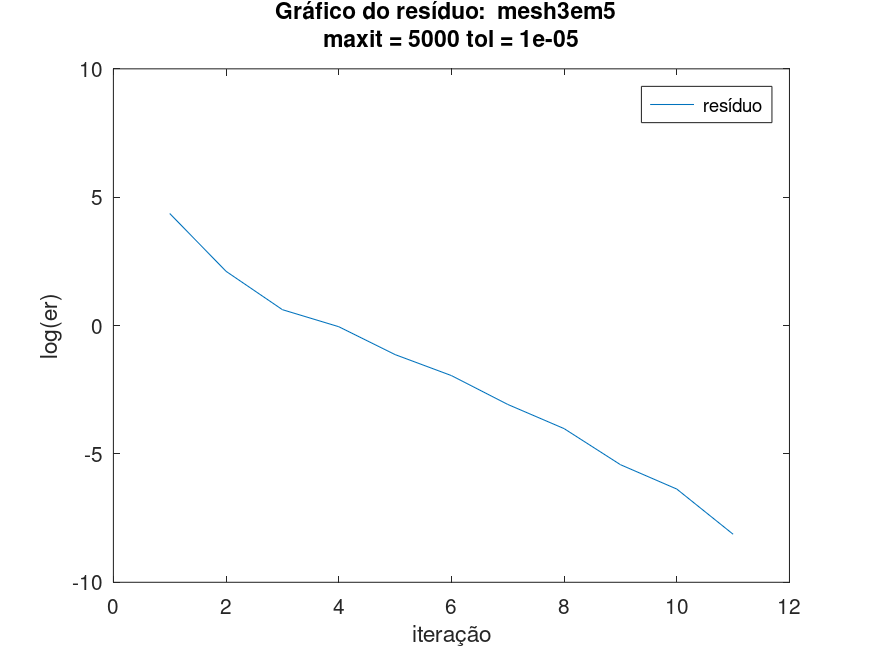
\includegraphics[width=\textwidth]{image/mesh3em5_5000_-6.png}
         \caption{Gráfico do Resíduo para maxit $= 5.000$ e tol $=10^{-6}$}
         \label{fig:mesh-5-6}
    \end{subfigure}
    \quad
    \begin{subfigure}[t]{0.36\linewidth}
         \centering
         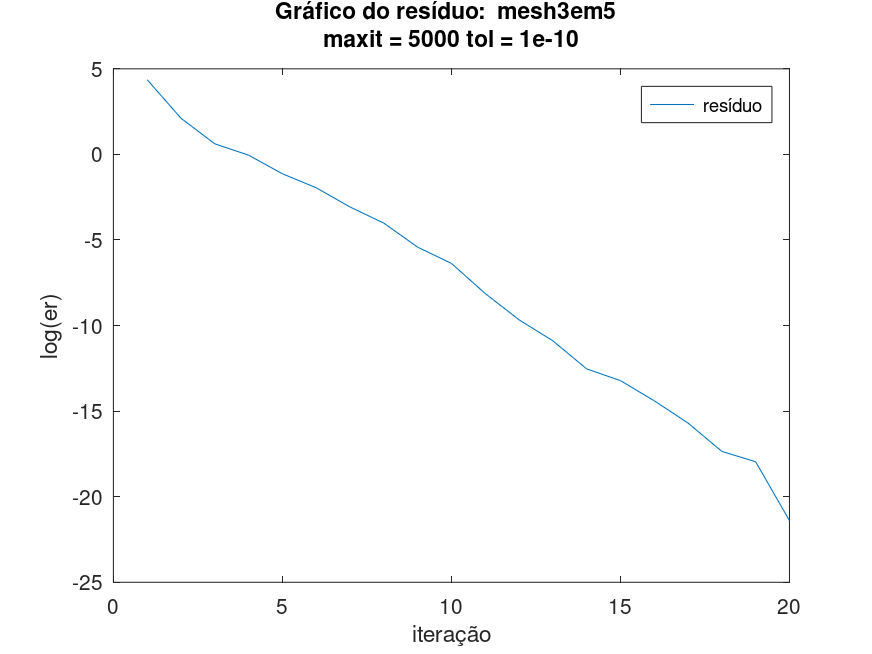
\includegraphics[width=\textwidth]{image/mesh3em5_5000_-11.png}
         \caption{Gráfico do Resíduo para maxit $= 5.000$ e tol $=10^{-11}$}
         \label{fig:mesh-5-11}
    \end{subfigure}
    \par\bigskip
    \begin{subfigure}[t]{0.36\linewidth}
         \centering
         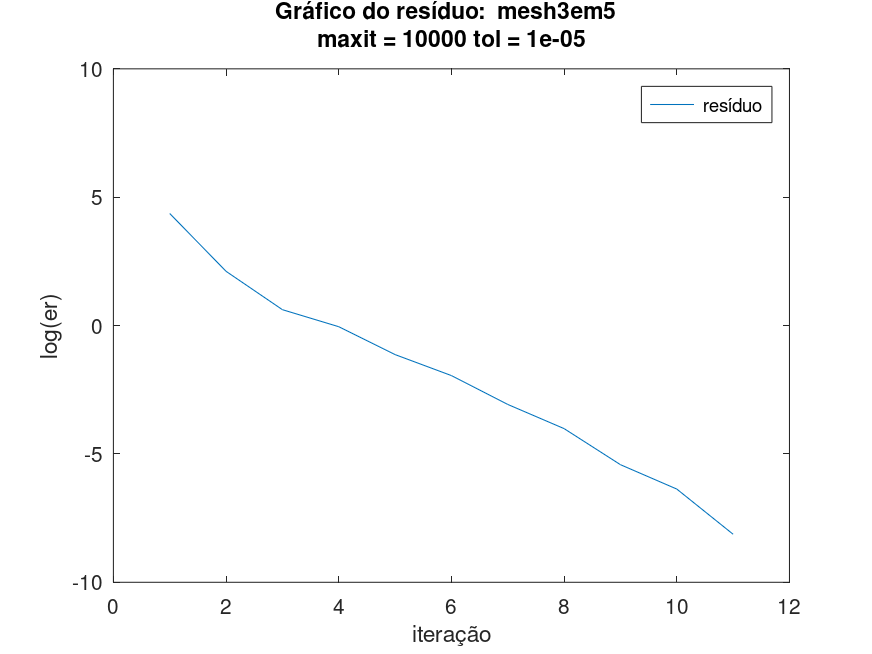
\includegraphics[width=\textwidth]{image/mesh3em5_10000_-6.png}
         \caption{Gráfico do Resíduo para maxit $= 10.000$ e tol $=10^{-6}$}
         \label{fig:mesh-10-6}
    \end{subfigure}
    \quad
    \begin{subfigure}[t]{0.36\linewidth}
         \centering
         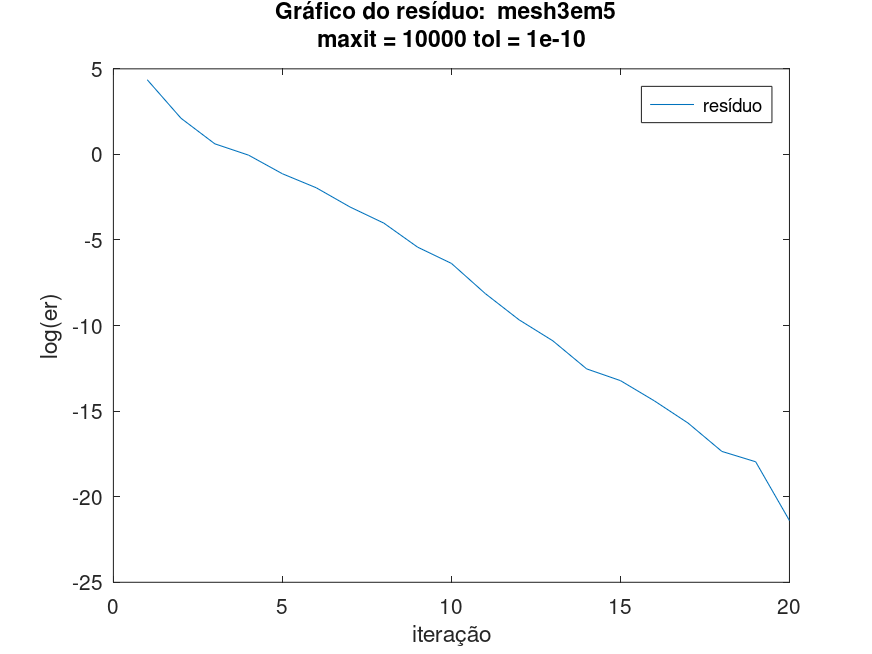
\includegraphics[width=\textwidth]{image/mesh3em5_10000_-11.png}
         \caption{Gráfico do Resíduo para maxit $= 10.000$ e tol $=10^{-11}$}
         \label{fig:mesh-10-11}
    \end{subfigure}
    \caption{Gráficos dos resíduos para \textit{mesh3em5}.}
    \label{fig:mesh}
\end{figure}